% vim: set foldmethod=marker foldlevel=0:

\documentclass[a4paper]{article}
\usepackage[UKenglish]{babel}

\usepackage{preamble}

\usepackage{graphicx}
\graphicspath{ {./imgs/} }

% \renewcommand{\thesubsection}{Q\thesection~(\alph{subsection})}

\fancyhead[L]{MA146 Assignment 3}
\title{MA146 Methods of Mathematical Modelling 1, Assignment 3}

\begin{document}

\maketitle

\setlength{\parindent}{0em}
\setlength{\parskip}{1em}

% {{{ Q1
\question{1}

Let $a, b, c, d \in \mathbb Z$. Then $$[d] = \left[ r^a v^b \rho^c \mu^d \right] = L^a L^b T^{-2b} M^c L^{-3c} M^d L^{-d} T^{-d} = MLT^{-2}$$

Then we get the simultaneous equations \begin{align*}
	c + d &= 1\\
	a + b - 3c - d &= 1\\
	-2b - d &= -2
\end{align*}

We don't have enough information to solve the system from here, but we can simplify to get \begin{align*}
	a &= 3 - \frac32 d\\
	b &= 1 - \frac d2\\
	c &= 1 - d
\end{align*}

Since they're all integers, we know that $d$ is even, so we can just try even values of $d$.

$d=2$ gives \begin{align*}
	a &= 0\\
	b &= 0\\
	c &= -1\\
	d &= 2\\
\end{align*}
But we want the radius and velocity to be part of the equation, so we don't want $a=b=0$.

$d=4$ gives \begin{align*}
	a &= -3\\
	b &= -1\\
	c &= -3\\
	d &= 4\\
\end{align*}

Therefore $[d] = \left[ r^{-3} v^{-1} \rho^{-3} \mu^4 \right]$.
% }}}

% {{{ Q2
\newquestion{2}

\subsection{~}

$$\dot x(t) = \frac{\alpha}{x(t)}$$

\subsection{~}

Let midnight be time $t = 0$, $t$ be in hours and $x(t)$ be in millimetres. Then $x(0) = 2$ and $x(4) = 3$.

\begin{align*}
	\frac{\mathrm d x}{\mathrm d t} &= \frac{\alpha}{x}\\
	\int x \mathrm d x              &= \int \alpha \mathrm d t\\
	\frac{x^2}{2}                   &= \alpha t + C\\
	\therefore x(t)                 &= \sqrt{2\alpha t + C}
\end{align*}

Then we can use the initial values.

\begin{align*}
	x(0) &= \sqrt{2 \alpha \times 0 + C}\\
		 &= \sqrt C\\
		 &= 2\\
	\implies C &= 4
\end{align*}

\begin{align*}
	x(2) &= \sqrt{2 \alpha \times 4 + 4}\\
		 &= 3\\
	\implies 8 \alpha &= 3^2 - 4\\
					  &= 5\\
	\implies \alpha &= \frac58\\
	\therefore x(t) &= \sqrt{\frac54 t + 4}
\end{align*}

Now we can just plug in 9:36 am, which is $9.6$ after midnight, and find that $x(9.6) = \sqrt{12 + 4} = 4$. Therefore the ice will be 4 mm thick at 9:36 am.

\subsection{~}

Now we have the differential equation $$\dot x(t) = \frac{\alpha \left(1 + \cos\left( \frac{\pi}{12} t \right)\right)}{x(t)}$$

We can solve this like before, \begin{align*}
	\frac{\mathrm d x}{\mathrm d t} &= \frac{\alpha \left(1 + \cos\left( \frac{\pi}{12} t \right)\right)}{x}\\[1ex]
	\int x \mathrm d x &= \int \alpha \left( 1 + \cos\left(\frac{\pi}{12} t\right) \right) \mathrm d t\\[1ex]
	\frac{x^2}{2} &= \alpha t + \alpha \frac{12}{\pi} \sin \left(\frac{\pi}{12} t\right) + C\\[1ex]
	\therefore x(t) &= \sqrt{2\alpha t + \frac{24\alpha}{\pi} \sin \left(\frac{\pi}{12} t\right) + C}
\end{align*}

Let $t_0 = 0$. Then $x(t_0) = x(0) = \sqrt{0 + \frac{24 \alpha}{\pi} \sin 0 + C} = \sqrt{C} = x_0$, therefore $C = (x_0)^2$.

Therefore, $$x(t) = \sqrt{2\alpha t + \frac{24\alpha}{\pi} \sin \left(\frac{\pi}{12} t\right) + (x_0)^2}$$
% }}}

% {{{ Q3
\newquestion{3}

\subsection{~}

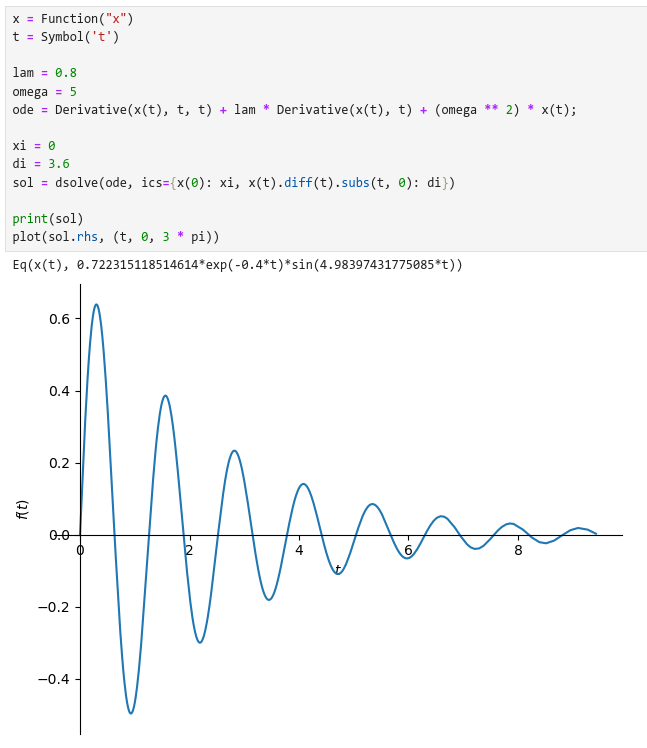
\includegraphics[scale=0.6]{Q3-a}

\subsection{~}

My solution is $n_\text{min} = 9$.

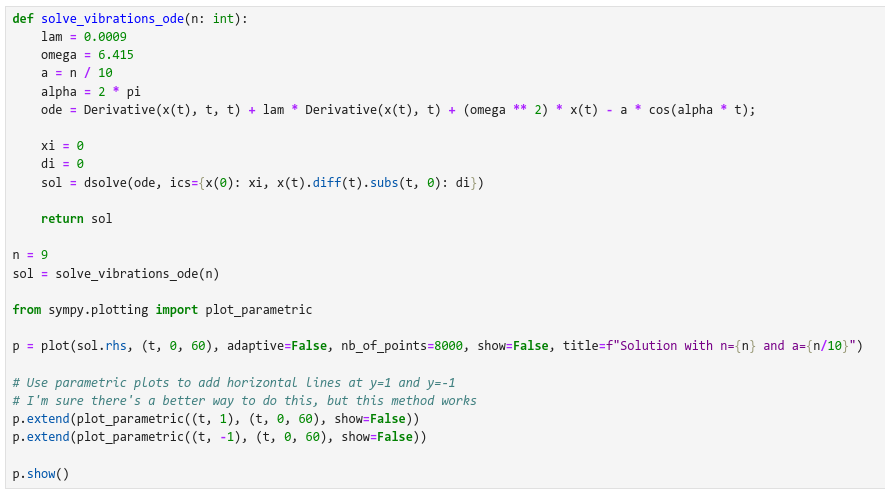
\includegraphics[scale=0.45]{Q3-b}
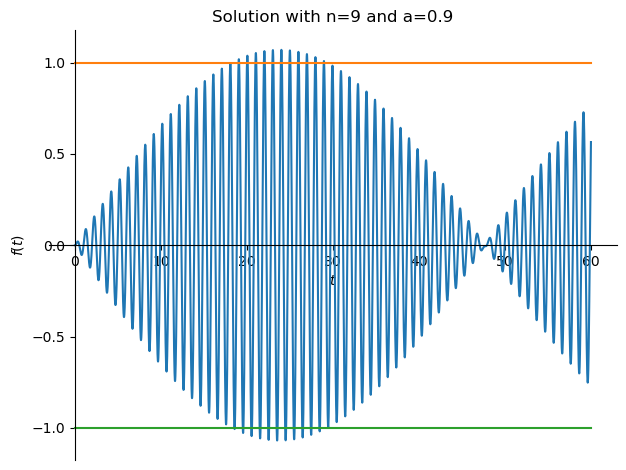
\includegraphics[scale=0.8]{n9}
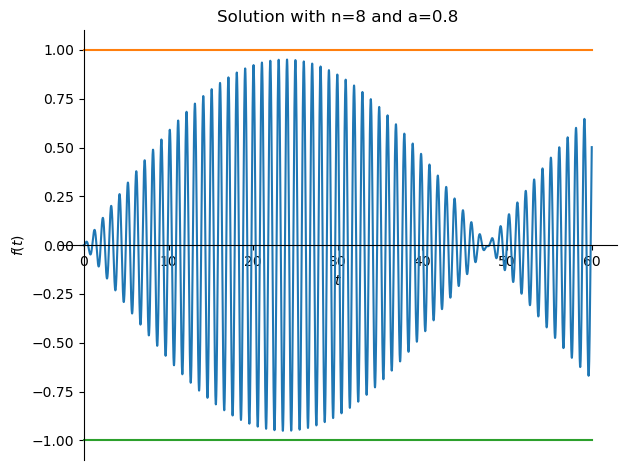
\includegraphics[scale=0.8]{n8}
% }}}

% {{{ Q4
\newquestion{4}

$$\frac{\mathrm d^2}{\mathrm d t^2} y(t) + \eta \frac{\mathrm d}{\mathrm d t} y(t) + b y(t) = f \cos(\theta t)$$

Since the right hand side is $f \cos(\theta t)$, we will use $y(t) = A \cos(\theta t) + B \sin(\theta t)$ as our particular integral.
\begin{align*}
	y(t)   &= A \cos(\theta t) + B \sin(\theta t)\\
	y'(t)  &= -\theta A \sin(\theta t) + \theta B \cos(\theta t)\\
	y''(t) &= -\theta^2 A \cos(\theta t) - \theta^2 B \sin(\theta t)
\end{align*}

Plugging this into the ODE, we get $$-\theta^2 A \cos(\theta t) - \theta^2 B \sin(\theta t) -\eta\theta A \sin(\theta t) + \eta\theta B \cos(\theta t) + bA \cos(\theta t) + bB \sin(\theta t) = f \cos(\theta t)$$

We can compare coefficients of $\sin$ and $\cos$ and conclude that \begin{align*}
	-\theta^2 B - \eta\theta A + bB &= 0\\
	-\theta^2 A - \eta\theta B + bA &= f
\end{align*}

The first equation implies $B(b - \theta^2) = \eta\theta A$. We can use this to get $B$ in terms of $A$, so $B = \dfrac{\eta\theta A}{b - \theta^2}$. Then we can plug that into the second equation, which gives $$A \left(-\theta^2 + \frac{\eta^2 \theta^2}{b - \theta^2} + b\right) = f$$

Therefore $$A = \frac{f (b - \theta^2)}{(b - \theta^2)^2 + \eta^2 \theta^2}$$

And therefore $$B = \frac{\eta \theta f}{(b - \theta^2)^2 + \eta^2 \theta^2}$$

Therefore the particular integral is $$\frac{f (b - \theta^2)}{(b - \theta^2)^2 + \eta^2 \theta^2} \cos(\theta t) + \frac{\eta \theta f}{(b - \theta^2)^2 + \eta^2 \theta^2} \sin (\theta t)$$

Alternatively written as $$\frac{f}{(b - \theta^2)^2 + \eta^2 \theta^2} \left( (b - \theta^2) \cos(\theta t) + \eta \theta \sin(\theta t) \right)$$
% }}}

\end{document}
